% !TEX TS-program = pdflatex
% !TEX encoding = UTF-8 Unicode

% This is a simple template for a LaTeX document using the "article" class.
% See "book", "report", "letter" for other types of document.

\documentclass[12pt]{article} % use larger type; default would be 10pt

\usepackage[utf8]{inputenc} % set input encoding (not needed with XeLaTeX)

%%% Examples of Article customizations
% These packages are optional, depending whether you want the features they provide.
% See the LaTeX Companion or other references for full information.

%%% PAGE DIMENSIONS
\usepackage{geometry} % to change the page dimensions
\geometry{a4paper} % or letterpaper (US) or a5paper or....
% \geometry{margin=2in} % for example, change the margins to 2 inches all round
% \geometry{landscape} % set up the page for landscape
%   read geometry.pdf for detailed page layout information

\usepackage{graphicx} % support the \includegraphics command and options

% \usepackage[parfill]{parskip} % Activate to begin paragraphs with an empty line rather than an indent

%%% PACKAGES
\usepackage{booktabs} % for much better looking tables
\usepackage{array} % for better arrays (eg matrices) in maths
\usepackage{paralist} % very flexible & customisable lists (eg. enumerate/itemize, etc.)
\usepackage{verbatim} % adds environment for commenting out blocks of text & for better verbatim
\usepackage{subfig} % make it possible to include more than one captioned figure/table in a single float
\usepackage{graphicx}
\usepackage[colorlinks, urlcolor=cyan, citecolor=red]{hyperref}
% These packages are all incorporated in the memoir class to one degree or another...

%%% HEADERS & FOOTERS
\usepackage{fancyhdr} % This should be set AFTER setting up the page geometry
\pagestyle{fancy} % options: empty , plain , fancy
\renewcommand{\headrulewidth}{0pt} % customise the layout...
\lhead{}\chead{}\rhead{}
\lfoot{}\cfoot{\thepage}\rfoot{}

%%% SECTION TITLE APPEARANCE
\usepackage{sectsty}

\usepackage{enumitem}

%%% ToC (table of contents) APPEARANCE
\usepackage[nottoc,notlof,notlot]{tocbibind} % Put the bibliography in the ToC
\usepackage[titles,subfigure]{tocloft} % Alter the style of the Table of Contents
\usepackage{dirtree}
\usepackage{authblk}
\renewcommand{\cftsecfont}{\rmfamily\mdseries\upshape}
\renewcommand{\cftsecpagefont}{\rmfamily\mdseries\upshape} % No bold!

%%% END Article customizations

%%% The "real" document content comes below...

\title{OCR Handwriting Project Report}
\author{Matthew Mulhall}
\affil{matthew.l.mulhall@uconn.edu}
%\date{} % Activate to display a given date or no date (if empty),

\begin{document}
\maketitle
This is a report outlining what has been achieved so far for this OCR-Handwriting Transcription project for the summer of 2019 from May-August. This serves as a basis for understanding of what the project has achieved as well as a basis for writing an papers or grant proposals.

\section{Technical Specifications}
\noindent\makebox[\linewidth]{\rule{15cm}{0.4pt}}
We currently have 7 documents that have been allocated for our project. The first 4 will be used to create the data set of images. On top of simple screenshots, we will also employ GPUs to transform the images to get the most mileage out of each photo. The last 3 will be later allocated into development and strict testing sets. These will be allocated as the training set is developed.

\subsection{Description of file system}
\dirtree{%
.1 OCR-Handwriting .
.2 bin .
.3 src .
.4 testing .
.3 data.
.4 char .
.5 ascii lower .
.6 a to z.
.5 ascii upper.
.6 A to Z.
.5 ascii number.
.6 0 to 9 .
.5 compound .
.5 punctuation .
.4 documents .
.5 Training Set.
.2 documentation .
.3 Project Log.
.3 Completion Log.
.2 utilities .
}
\begin{enumerate}[label = (\roman*)]
\item Bin contains all of the 'raw' data such as images, and documents where the images come from. Each sub directory is ordered.
\item The section 'compound' has been added due to the nature of John Quincy Adams handwriting. There are several small phrases like 'Mr' and 'Dr' that appear more as one character than 2. This is why it is denoted as 'compound', meaning more than one letter interpreted as a single unit.
\item Documentation contains this document, as well as any other documents that are needed to explain the project.
\item Utilities contains all scripts, programs, or software that we use as a supplement in order to complete the project.
\end{enumerate}

\subsection{Software Information}
\begin{enumerate}[label = (\roman*)]
\item Python 3.7.3
\item Github
\item \textbf{Packages:}
\item Keras
\item Tensorflow/Tensorflow-gpu
\item NumPY
\item cv2 (OpenCV)
\item imutils
\item GraphViz
\item Matplotlib
\item PyDot
\item AutoAiLib - Library that was formed after noticing key gripes while developing the ML models. The library is a small collection of testing classes, data manipulation classes, as well as pure functions that make creating ML easier.
\end{enumerate}

\section{Models}
\noindent\makebox[\linewidth]{\rule{15cm}{0.4pt}}
Over the course of the summer the project has accumulated 41 models from the time of writing this report. Almost all models built upon the previous successful model and furthered that sucess. Even with our minimal amounts of data we have been able to achieve 96\% + success rate for 4 way identification, and 86\% + accuracy on 22 class identification.


\section{Data}
\noindent\makebox[\linewidth]{\rule{15cm}{0.4pt}}
This project has amassed 16,000+ images of characters throughout the course of several months This averages out to 260 images per class. Historically speaking this is a very low amount of representative data for convolutional neural networks. Despite this, we have been able to get good results out of our models. Even so, I posit that to make enterprise level sofftware we will require data increases by a factor of 3-5x. We completed tests earlier in order to see what type of correlation we found between a class' sucess rate when plotted against its data size.
The following is a graph showing the total number of samples vs correct guesses that was achieved during a test on the 7th iteration of the medium set model.

\section{Testing}
\noindent\makebox[\linewidth]{\rule{15cm}{0.4pt}}
\begin{enumerate}[label = (\roman*)]
\item In order to gauge the effect of increasing size relative to a single sample rather than a change in sample classes (as was done in the previous test), we chose to expand a data set through manual augmentation and comparing it to the same, unaugmented set.
\item We went back to the original smallset test, which has 4 classes with 1,539 images. Through a program called image transform  that I wrote, I augmented them and got 3,053 images total from the base set.
\item Examples of augmentation:
\item 
\includegraphics{{augmented/augmented_6}} 
\includegraphics{{augmented/augmented_61}} 
\includegraphics{{augmented/augmented_73}} 
\includegraphics{{augmented/augmented_87}}
\item The results were as follows:
\item Baseline:
\item 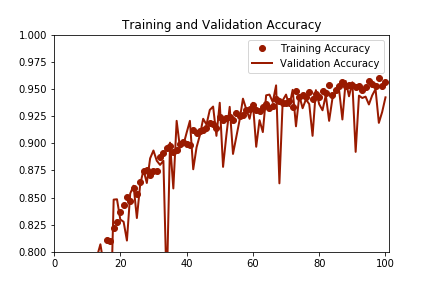
\includegraphics{{new_med_imgs/acc_historybaseline}}
\item 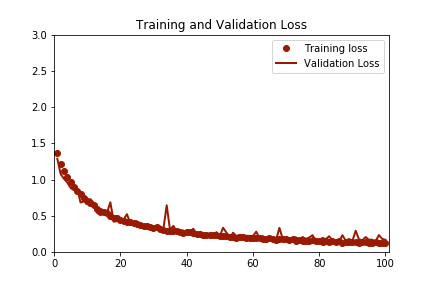
\includegraphics{{new_med_imgs/loss_historybaseline}}
\item Test:
\item 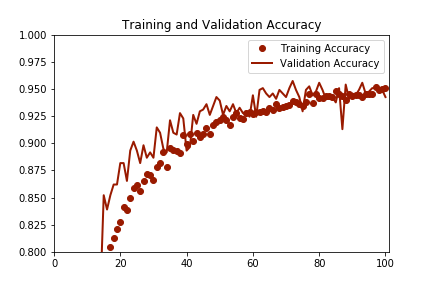
\includegraphics{{new_med_imgs/acc_historytest}}
\item 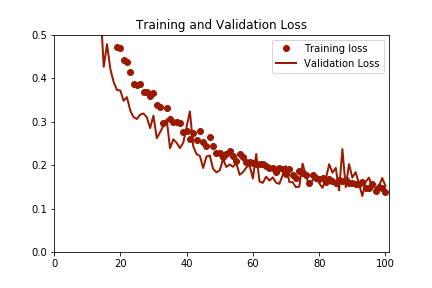
\includegraphics{{new_med_imgs/loss_historytest}}
\item The results are inconclusive , although the decrease in loss is notable. As can be seen in Figure VII there appears to be a small uptick in accuracy at the end of the training cycle. We intend to test what happens with slightly increased training to 150 epochs.
\item Results:
\item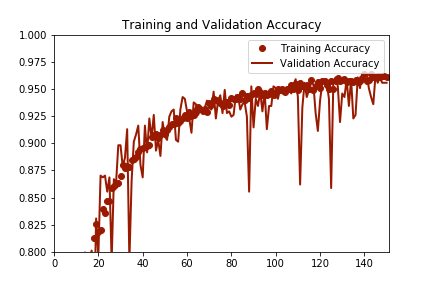
\includegraphics{{new_med_imgs/acc_historytest150epochs}}
\item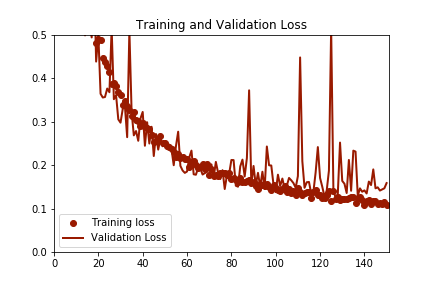
\includegraphics{{new_med_imgs/loss_historytest150epochs}}
\item After these tests were performed I moved onto to testing the larger class set, and plot identification rate vs data examples for a clearer conclusion. 
\item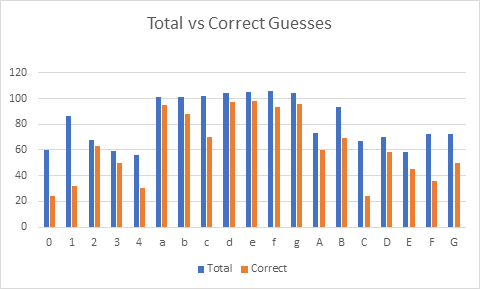
\includegraphics{charts/total-vs-correct}
\item The following graphic used the previous graphs data to find the relationship between sample sizes and correctness.
\item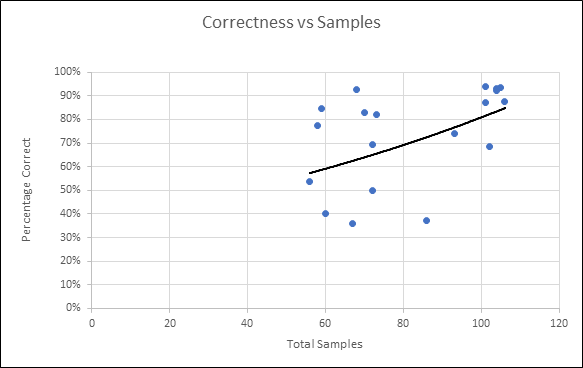
\includegraphics {charts/correct-vs-samples}
\end{enumerate}
Given the conclusions of the tests as well as plotting the information into graphs, the model needs more data. The previous chart's trendline clearly suggests that there is a positive relationship between samples taken and the model's success. Although this seems obvious, it was important to isolate each character, as well as rule out the interaction of certain characters. I.e. it was important to figure out if 'b' and 'd' interacted, or if they had high success despite their similarity. However, we have seen lower success than usual for 'b' in some tests, most likely due to focusing on smaller feature extraction in those models. From what I can deduce from our tests, it is useful to have strides be centrally distributed, meaning: 1-2 (1,1) , 1-2 (5,5), 1 (7,7), and mostly (3,3). This seems to be a winning combination in these CNNs. This is most likely due to the fact that the features between each image that are different are not large or small, but 'medium' as strange as that language sounds. This distribution however gives our model the opportunity to pick up on all possible differences and train for them.



\section{Conclusions}
\noindent\makebox[\linewidth]{\rule{15cm}{0.4pt}}
\begin{enumerate}[label = (\roman*)]
\item Given the data shown the models have reached a point where they are as good as they can get with the data we have. In order to further push the models, and eventually scale up to 70+ classes, we will need more example images. As prviously stated, a good aim would be 3-5x increase in data, and then performing more tests.
\end{enumerate}



\end{document}